% Figure 8: ARE Throughput vs Step Count
\documentclass[tikz,border=5pt]{standalone}
\usepackage{pgfplots}
\pgfplotsset{compat=1.18}

\begin{document}
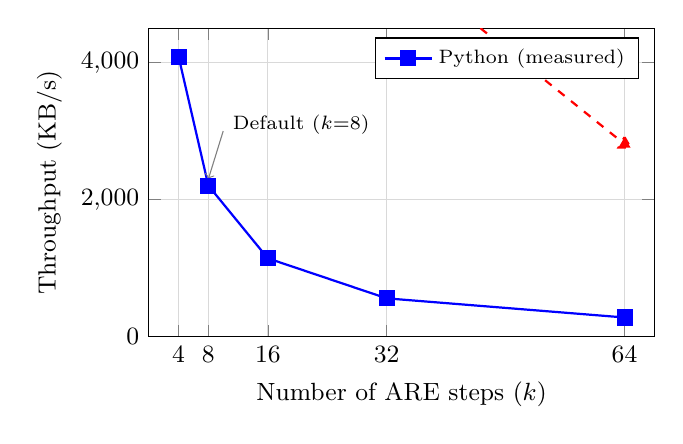
\begin{tikzpicture}
\begin{axis}[
  width=8cm, height=5.5cm,
  xlabel={Number of ARE steps ($k$)},
  ylabel={Throughput (KB/s)},
  xmin=0, xmax=68,
  ymin=0, ymax=4500,
  xtick={4,8,16,32,64},
  grid=major,
  grid style={gray!30},
  legend pos=north east,
  legend style={font=\scriptsize},
  font=\small,
]

% Python throughput (measured)
\addplot[thick, blue, mark=square*, mark size=2.5pt] coordinates {
  (4, 4085)
  (8, 2205)
  (16, 1144)
  (32, 560)
  (64, 281)
};
\addlegendentry{Python (measured)}

% Estimated Rust (10x speedup, conservative)
\addplot[thick, red, dashed, mark=triangle*, mark size=2.5pt] coordinates {
  (4, 40850)
  (8, 22050)
  (16, 11440)
  (32, 5600)
  (64, 2810)
};
% Don't show Rust in plot area (would compress Python line)
% \addlegendentry{Rust (est. 10x)}

% Annotation for default config
\draw[->, gray] (axis cs:10, 3000) -- (axis cs:8, 2300);
\node[font=\scriptsize, anchor=west] at (axis cs:10, 3100) {Default ($k{=}8$)};

\end{axis}
\end{tikzpicture}
\end{document}
